% Options for packages loaded elsewhere
\PassOptionsToPackage{unicode}{hyperref}
\PassOptionsToPackage{hyphens}{url}
%
\documentclass[
]{book}
\usepackage{amsmath,amssymb}
\usepackage{lmodern}
\usepackage{iftex}
\ifPDFTeX
  \usepackage[T1]{fontenc}
  \usepackage[utf8]{inputenc}
  \usepackage{textcomp} % provide euro and other symbols
\else % if luatex or xetex
  \usepackage{unicode-math}
  \defaultfontfeatures{Scale=MatchLowercase}
  \defaultfontfeatures[\rmfamily]{Ligatures=TeX,Scale=1}
\fi
% Use upquote if available, for straight quotes in verbatim environments
\IfFileExists{upquote.sty}{\usepackage{upquote}}{}
\IfFileExists{microtype.sty}{% use microtype if available
  \usepackage[]{microtype}
  \UseMicrotypeSet[protrusion]{basicmath} % disable protrusion for tt fonts
}{}
\makeatletter
\@ifundefined{KOMAClassName}{% if non-KOMA class
  \IfFileExists{parskip.sty}{%
    \usepackage{parskip}
  }{% else
    \setlength{\parindent}{0pt}
    \setlength{\parskip}{6pt plus 2pt minus 1pt}}
}{% if KOMA class
  \KOMAoptions{parskip=half}}
\makeatother
\usepackage{xcolor}
\IfFileExists{xurl.sty}{\usepackage{xurl}}{} % add URL line breaks if available
\IfFileExists{bookmark.sty}{\usepackage{bookmark}}{\usepackage{hyperref}}
\hypersetup{
  pdftitle={HW3: Group Project GitHub + Bookdown Setup},
  pdfauthor={Coded in COBOL},
  hidelinks,
  pdfcreator={LaTeX via pandoc}}
\urlstyle{same} % disable monospaced font for URLs
\usepackage{color}
\usepackage{fancyvrb}
\newcommand{\VerbBar}{|}
\newcommand{\VERB}{\Verb[commandchars=\\\{\}]}
\DefineVerbatimEnvironment{Highlighting}{Verbatim}{commandchars=\\\{\}}
% Add ',fontsize=\small' for more characters per line
\usepackage{framed}
\definecolor{shadecolor}{RGB}{248,248,248}
\newenvironment{Shaded}{\begin{snugshade}}{\end{snugshade}}
\newcommand{\AlertTok}[1]{\textcolor[rgb]{0.94,0.16,0.16}{#1}}
\newcommand{\AnnotationTok}[1]{\textcolor[rgb]{0.56,0.35,0.01}{\textbf{\textit{#1}}}}
\newcommand{\AttributeTok}[1]{\textcolor[rgb]{0.77,0.63,0.00}{#1}}
\newcommand{\BaseNTok}[1]{\textcolor[rgb]{0.00,0.00,0.81}{#1}}
\newcommand{\BuiltInTok}[1]{#1}
\newcommand{\CharTok}[1]{\textcolor[rgb]{0.31,0.60,0.02}{#1}}
\newcommand{\CommentTok}[1]{\textcolor[rgb]{0.56,0.35,0.01}{\textit{#1}}}
\newcommand{\CommentVarTok}[1]{\textcolor[rgb]{0.56,0.35,0.01}{\textbf{\textit{#1}}}}
\newcommand{\ConstantTok}[1]{\textcolor[rgb]{0.00,0.00,0.00}{#1}}
\newcommand{\ControlFlowTok}[1]{\textcolor[rgb]{0.13,0.29,0.53}{\textbf{#1}}}
\newcommand{\DataTypeTok}[1]{\textcolor[rgb]{0.13,0.29,0.53}{#1}}
\newcommand{\DecValTok}[1]{\textcolor[rgb]{0.00,0.00,0.81}{#1}}
\newcommand{\DocumentationTok}[1]{\textcolor[rgb]{0.56,0.35,0.01}{\textbf{\textit{#1}}}}
\newcommand{\ErrorTok}[1]{\textcolor[rgb]{0.64,0.00,0.00}{\textbf{#1}}}
\newcommand{\ExtensionTok}[1]{#1}
\newcommand{\FloatTok}[1]{\textcolor[rgb]{0.00,0.00,0.81}{#1}}
\newcommand{\FunctionTok}[1]{\textcolor[rgb]{0.00,0.00,0.00}{#1}}
\newcommand{\ImportTok}[1]{#1}
\newcommand{\InformationTok}[1]{\textcolor[rgb]{0.56,0.35,0.01}{\textbf{\textit{#1}}}}
\newcommand{\KeywordTok}[1]{\textcolor[rgb]{0.13,0.29,0.53}{\textbf{#1}}}
\newcommand{\NormalTok}[1]{#1}
\newcommand{\OperatorTok}[1]{\textcolor[rgb]{0.81,0.36,0.00}{\textbf{#1}}}
\newcommand{\OtherTok}[1]{\textcolor[rgb]{0.56,0.35,0.01}{#1}}
\newcommand{\PreprocessorTok}[1]{\textcolor[rgb]{0.56,0.35,0.01}{\textit{#1}}}
\newcommand{\RegionMarkerTok}[1]{#1}
\newcommand{\SpecialCharTok}[1]{\textcolor[rgb]{0.00,0.00,0.00}{#1}}
\newcommand{\SpecialStringTok}[1]{\textcolor[rgb]{0.31,0.60,0.02}{#1}}
\newcommand{\StringTok}[1]{\textcolor[rgb]{0.31,0.60,0.02}{#1}}
\newcommand{\VariableTok}[1]{\textcolor[rgb]{0.00,0.00,0.00}{#1}}
\newcommand{\VerbatimStringTok}[1]{\textcolor[rgb]{0.31,0.60,0.02}{#1}}
\newcommand{\WarningTok}[1]{\textcolor[rgb]{0.56,0.35,0.01}{\textbf{\textit{#1}}}}
\usepackage{longtable,booktabs,array}
\usepackage{calc} % for calculating minipage widths
% Correct order of tables after \paragraph or \subparagraph
\usepackage{etoolbox}
\makeatletter
\patchcmd\longtable{\par}{\if@noskipsec\mbox{}\fi\par}{}{}
\makeatother
% Allow footnotes in longtable head/foot
\IfFileExists{footnotehyper.sty}{\usepackage{footnotehyper}}{\usepackage{footnote}}
\makesavenoteenv{longtable}
\usepackage{graphicx}
\makeatletter
\def\maxwidth{\ifdim\Gin@nat@width>\linewidth\linewidth\else\Gin@nat@width\fi}
\def\maxheight{\ifdim\Gin@nat@height>\textheight\textheight\else\Gin@nat@height\fi}
\makeatother
% Scale images if necessary, so that they will not overflow the page
% margins by default, and it is still possible to overwrite the defaults
% using explicit options in \includegraphics[width, height, ...]{}
\setkeys{Gin}{width=\maxwidth,height=\maxheight,keepaspectratio}
% Set default figure placement to htbp
\makeatletter
\def\fps@figure{htbp}
\makeatother
\setlength{\emergencystretch}{3em} % prevent overfull lines
\providecommand{\tightlist}{%
  \setlength{\itemsep}{0pt}\setlength{\parskip}{0pt}}
\setcounter{secnumdepth}{5}
\usepackage{booktabs}
\ifLuaTeX
  \usepackage{selnolig}  % disable illegal ligatures
\fi
\usepackage[]{natbib}
\bibliographystyle{plainnat}

\title{HW3: Group Project GitHub + Bookdown Setup}
\author{Coded in COBOL}
\date{2022-07-25}

\usepackage{amsthm}
\newtheorem{theorem}{Theorem}[chapter]
\newtheorem{lemma}{Lemma}[chapter]
\newtheorem{corollary}{Corollary}[chapter]
\newtheorem{proposition}{Proposition}[chapter]
\newtheorem{conjecture}{Conjecture}[chapter]
\theoremstyle{definition}
\newtheorem{definition}{Definition}[chapter]
\theoremstyle{definition}
\newtheorem{example}{Example}[chapter]
\theoremstyle{definition}
\newtheorem{exercise}{Exercise}[chapter]
\theoremstyle{definition}
\newtheorem{hypothesis}{Hypothesis}[chapter]
\theoremstyle{remark}
\newtheorem*{remark}{Remark}
\newtheorem*{solution}{Solution}
\begin{document}
\maketitle

{
\setcounter{tocdepth}{1}
\tableofcontents
}
\hypertarget{table-of-contents}{%
\chapter{Table of Contents}\label{table-of-contents}}

\textbf{2. Introduction}

\textbf{3. About Us}

\begin{itemize}
\tightlist
\item
  3.1 Yuchen
\item
  3.2 Nikita
\item
  3.3 Ben
\item
  3.4 Peiyue
\item
  3.5 Winnifer
\item
  3.6 Jalal
\end{itemize}

\hypertarget{introduction}{%
\chapter{Introduction}\label{introduction}}

We are Coded in Cobol. Our proposal is to create a detailed e-guide for newly admitted MBAn students. This guide can help students get familiar with the campus environment and make full use of the resources around them effectively.

In class yesterday we talked with you about the fact that multiple groups are pursuing a similar idea. We plan to meet with these groups after submitting the proposal to split the tasks into three parts and then combine our three websites into one big website. Some specifics on the things we want to cover are:

\hypertarget{what-we-plan-to-cover}{%
\section{What We Plan to Cover}\label{what-we-plan-to-cover}}

\begin{itemize}
\tightlist
\item
  Dining plan/meal prep tips
\item
  Best local restaurants and bars
\item
  Fun things to do
\item
  Technology tips
\item
  Most Instagrammable Spots In Michigan
\item
  Transportation Tips
\item
  Study Spots
\item
  Sports
\end{itemize}

\hypertarget{cross}{%
\chapter{Cross-references}\label{cross}}

Cross-references make it easier for your readers to find and link to elements in your book.

\hypertarget{chapters-and-sub-chapters}{%
\section{Chapters and sub-chapters}\label{chapters-and-sub-chapters}}

There are two steps to cross-reference any heading:

\begin{enumerate}
\def\labelenumi{\arabic{enumi}.}
\tightlist
\item
  Label the heading: \texttt{\#\ Hello\ world\ \{\#nice-label\}}.

  \begin{itemize}
  \tightlist
  \item
    Leave the label off if you like the automated heading generated based on your heading title: for example, \texttt{\#\ Hello\ world} = \texttt{\#\ Hello\ world\ \{\#hello-world\}}.
  \item
    To label an un-numbered heading, use: \texttt{\#\ Hello\ world\ \{-\#nice-label\}} or \texttt{\{\#\ Hello\ world\ .unnumbered\}}.
  \end{itemize}
\item
  Next, reference the labeled heading anywhere in the text using \texttt{\textbackslash{}@ref(nice-label)}; for example, please see Chapter \ref{cross}.

  \begin{itemize}
  \tightlist
  \item
    If you prefer text as the link instead of a numbered reference use: \protect\hyperlink{cross}{any text you want can go here}.
  \end{itemize}
\end{enumerate}

\hypertarget{captioned-figures-and-tables}{%
\section{Captioned figures and tables}\label{captioned-figures-and-tables}}

Figures and tables \emph{with captions} can also be cross-referenced from elsewhere in your book using \texttt{\textbackslash{}@ref(fig:chunk-label)} and \texttt{\textbackslash{}@ref(tab:chunk-label)}, respectively.

See Figure \ref{fig:nice-fig}.

\begin{Shaded}
\begin{Highlighting}[]
\FunctionTok{par}\NormalTok{(}\AttributeTok{mar =} \FunctionTok{c}\NormalTok{(}\DecValTok{4}\NormalTok{, }\DecValTok{4}\NormalTok{, .}\DecValTok{1}\NormalTok{, .}\DecValTok{1}\NormalTok{))}
\FunctionTok{plot}\NormalTok{(pressure, }\AttributeTok{type =} \StringTok{\textquotesingle{}b\textquotesingle{}}\NormalTok{, }\AttributeTok{pch =} \DecValTok{19}\NormalTok{)}
\end{Highlighting}
\end{Shaded}

\begin{figure}

{\centering \includegraphics[width=0.8\linewidth]{_main_files/figure-latex/nice-fig-1} 

}

\caption{Here is a nice figure!}\label{fig:nice-fig}
\end{figure}

Don't miss Table \ref{tab:nice-tab}.

\begin{Shaded}
\begin{Highlighting}[]
\NormalTok{knitr}\SpecialCharTok{::}\FunctionTok{kable}\NormalTok{(}
  \FunctionTok{head}\NormalTok{(pressure, }\DecValTok{10}\NormalTok{), }\AttributeTok{caption =} \StringTok{\textquotesingle{}Here is a nice table!\textquotesingle{}}\NormalTok{,}
  \AttributeTok{booktabs =} \ConstantTok{TRUE}
\NormalTok{)}
\end{Highlighting}
\end{Shaded}

\begin{table}

\caption{\label{tab:nice-tab}Here is a nice table!}
\centering
\begin{tabular}[t]{rr}
\toprule
temperature & pressure\\
\midrule
0 & 0.0002\\
20 & 0.0012\\
40 & 0.0060\\
60 & 0.0300\\
80 & 0.0900\\
\addlinespace
100 & 0.2700\\
120 & 0.7500\\
140 & 1.8500\\
160 & 4.2000\\
180 & 8.8000\\
\bottomrule
\end{tabular}
\end{table}

\hypertarget{about-us}{%
\chapter{About Us}\label{about-us}}

In this section you can get to know more about the members of Coded in COBOL.

\hypertarget{yuchen-gao}{%
\section{Yuchen Gao}\label{yuchen-gao}}

Hello! My name is Yuchen Gao. I'm currently a master student pursuing a \href{https://michiganross.umich.edu/graduate/master-of-business-analytics}{MBAn} degree from the Ross School of Business at the University of Michigan. I have an undergraduate degree in Information Science from the \href{https://www.si.umich.edu/}{School of Information} at the University of Michigan.

I am passionate about transforming data into impactful business solutions and would hope to work in the analytics field after getting my master's degree.

\includegraphics[width=0.5\textwidth,height=\textheight]{DSC00610.jpg}

\textbf{My favorite quote}
\textgreater{} ``All models are wrong, but some are useful''\\
\textgreater{} George E.P. Box

\textbf{Interests and Hobbies}
- I spent the first 18 years of my life in Shanghai, but I also lived in Boston for two years before coming to Ann Arbor, MI.
- In my free time I like to play tennis. I'm currently trying to improve my backhand and serving.
- I'm a big fan of electronic music. My most favorite genres are techno house, future house, future bass.
- My favorite novel is Neuromancer by William Gibson.
- I'm a coffee enthusiast. My favorite kind of coffee bean is Panama Geisha. If you happen to go to any coffee shop that is offering Geisha I highly recommend you to try it.

\textbf{More about Me\ldots{}}
You can find more information about my professional experiences on \href{https://www.linkedin.com/in/ycg2022/}{LinkedIn} and check out my past coding projects on \href{https://github.com/Yuchen-G}{Github}.

\hypertarget{nikita-mamidi}{%
\section{Nikita Mamidi}\label{nikita-mamidi}}

\textbf{I'm Nikita Mamidi 😃}

\begin{center}\rule{0.5\linewidth}{0.5pt}\end{center}

\includegraphics[width=9.375in,height=4.6875in]{nikita1.png}

\textbf{A little bit about me:}

I graduated from the University of Illinois at Urbana Champaign with a BS in Econometrics and Quantitative Economics. I look back fondly on my undergrad days where I was an Ambassador for the amazing Economics department, the Head Teaching Assistant for a Business Statistics Course and a Senior Associate at Illinois Business Consulting. \textbf{GO ILLINI!}

In today's world organizations are coming up with so many fascinating data and tech driven solutions to previously insurmountable problems. I want to be part of such a force that impacts the world positively. To achieve those high-level data science skills, I recently started my Masters of Business Analytics at the Ross School of Business!

\includegraphics[width=4.6875in,height=3.64583in]{nikita3.jpeg} \includegraphics[width=4.6875in,height=3.64583in]{nikita2.png}

\begin{center}\rule{0.5\linewidth}{0.5pt}\end{center}

\textbf{Recent Work Experience:}

MSN Pharmaceuticals :- Sales and Marketing Executive

\begin{itemize}
\tightlist
\item
  Responsible for the South Korean, Japanese, Indonesian, Thailand and Taiwanese markets
\item
  Determined potential partnerships in East Asia, established contacts \& built relationships with key decision makers
\item
  Collaborated with technical teams to ensure production and distribution of high-quality samples and final API
\item
  Achieved the \textbf{\$3 million per month} revenue target for the past 2 quarters
\end{itemize}

\begin{center}\rule{0.5\linewidth}{0.5pt}\end{center}

\textbf{Fun Facts:}

\includegraphics[width=3.33333in,height=3.64583in]{nikita4.jpeg} \includegraphics[width=5.20833in,height=3.64583in]{nikita5.jpeg}

\begin{itemize}
\tightlist
\item
  I love to travel. Been to 20 countries. Next Destination - Mexico 🇲🇽
\item
  Stock market trading is everything! I'm a day trader tho, I know I'm awful 🤭
\item
  Certified online shopaholic. But I also return the goods with equal speed
\item
  I love watching (and dreaming of playing) in the NBA
\item
  I enjoy snorkeling and scuba diving
\item
  I'm terrified of all animals. Yes, including cute puppies and kittens 🤯
\end{itemize}

\textbf{That's enough about me 😁. Please reach out so I can learn more about You!}

\href{https://www.linkedin.com/in/nikita-mamidi-763b80185/}{Linkedin}

Contact - 217-898-6828

\hypertarget{ben-newman}{%
\section{Ben Newman}\label{ben-newman}}

\begin{quote}
Team: Coded in COBOL
\end{quote}

Bio: Hi, I'm Ben. I was raised in Midland, MI. It's in the middle-right part of the mitten. In high school, I was on the swim team (see below) and did cross country. I also attended University of Michigan from which I graduated last year (see below). Some things that bring joy to my life are friends, family, my pets (see below), skiing, fishing, and going to Michigan Football Games!!

\textbf{My Education}

\begin{itemize}
\tightlist
\item
  Saint Brigid Catholic School (Midland, MI USA)
\item
  Herbert Henry Dow High School (Midland, MI USA)
\item
  University of Michigan Ann Arbor (Ann Arbor, MI USA)

  \begin{itemize}
  \tightlist
  \item
    B.S. Statistics
  \end{itemize}
\item
  University of Michigan Ann Arbor (Ann Arbor, MI USA)

  \begin{itemize}
  \tightlist
  \item
    Masters in Business Analytics
  \end{itemize}
\end{itemize}

\textbf{My favorite foods.}

\begin{enumerate}
\def\labelenumi{\arabic{enumi}.}
\tightlist
\item
  Pizza
\item
  Orange Chicken
\item
  Burgers
\end{enumerate}

\includegraphics[width=0.25\textwidth,height=\textheight]{swimmers.jpg}

\begin{quote}
A picture of me (left) in my more fit days on the swim team (circa 2017).
\end{quote}

\includegraphics[width=0.25\textwidth,height=\textheight]{dogs.jpeg}

\begin{quote}
A picture of my dogs Pearl (left) and Blue (right). They are Weimaraners.
\end{quote}

\includegraphics[width=0.25\textwidth,height=\textheight]{Graduation.jpg}

\begin{quote}
This is me at the University of Michigan Commencement with my family in April, 2022.
\end{quote}

\hypertarget{peiyue-sun}{%
\section{Peiyue Sun}\label{peiyue-sun}}

This is Peiyue Sun.

\begin{itemize}
\tightlist
\item
  I love Michigan Wolverines!
\item
  I love Wisconsin Badgers!
\end{itemize}

Education:

\begin{itemize}
\tightlist
\item
  Wisconsin School of Business 2016 -\textgreater{} 2019 Risk Management \& Insurance (BBA)
\item
  Ross School of Business 2022 -\textgreater{} 2023 Business Analytics (MBAn)
\end{itemize}

Technology used:

\begin{itemize}
\tightlist
\item
  R
\item
  Python
\item
  Excel
\end{itemize}

Work Experience:

\begin{itemize}
\tightlist
\item
  2 years at Willis Towers Watson risk consulting sector

  \begin{itemize}
  \tightlist
  \item
    Insurance-linked securities valuation
  \item
    Financial Reserving for global insurance enterprises
  \end{itemize}
\end{itemize}

Goal at MBAN:

\begin{itemize}
\tightlist
\item
  Unlock my potential in business analytics and project management
\end{itemize}

Hobbies:

\begin{itemize}
\tightlist
\item
  Snooker, Basketball, Texas Hold'em, Swimming, Running, Biking, and Trap music festivals
\end{itemize}

\includegraphics[width=2.66667in,height=\textheight]{1.jpg}

\hypertarget{winnifer-chen}{%
\section{Winnifer Chen}\label{winnifer-chen}}

Winnifer Chen

Email: \href{mailto:winnifer@umich.edu}{\nolinkurl{winnifer@umich.edu}}

Phone: (980) 298-7184

LinkedIn: \url{https://www.linkedin.com/in/winnifer/}

\textbf{Educational Background}
I recently graduated with a Bachelor of Science in Economics with a minor in Statistics from the University of Michigan in April 2022. Currently, I am pursuing a Master of Business Analytics at the University of Michigan - Stephen M. Ross School of Business, with an expected graduation date of April 2023.

\includegraphics[width=0.25\textwidth,height=\textheight]{grad.JPG}
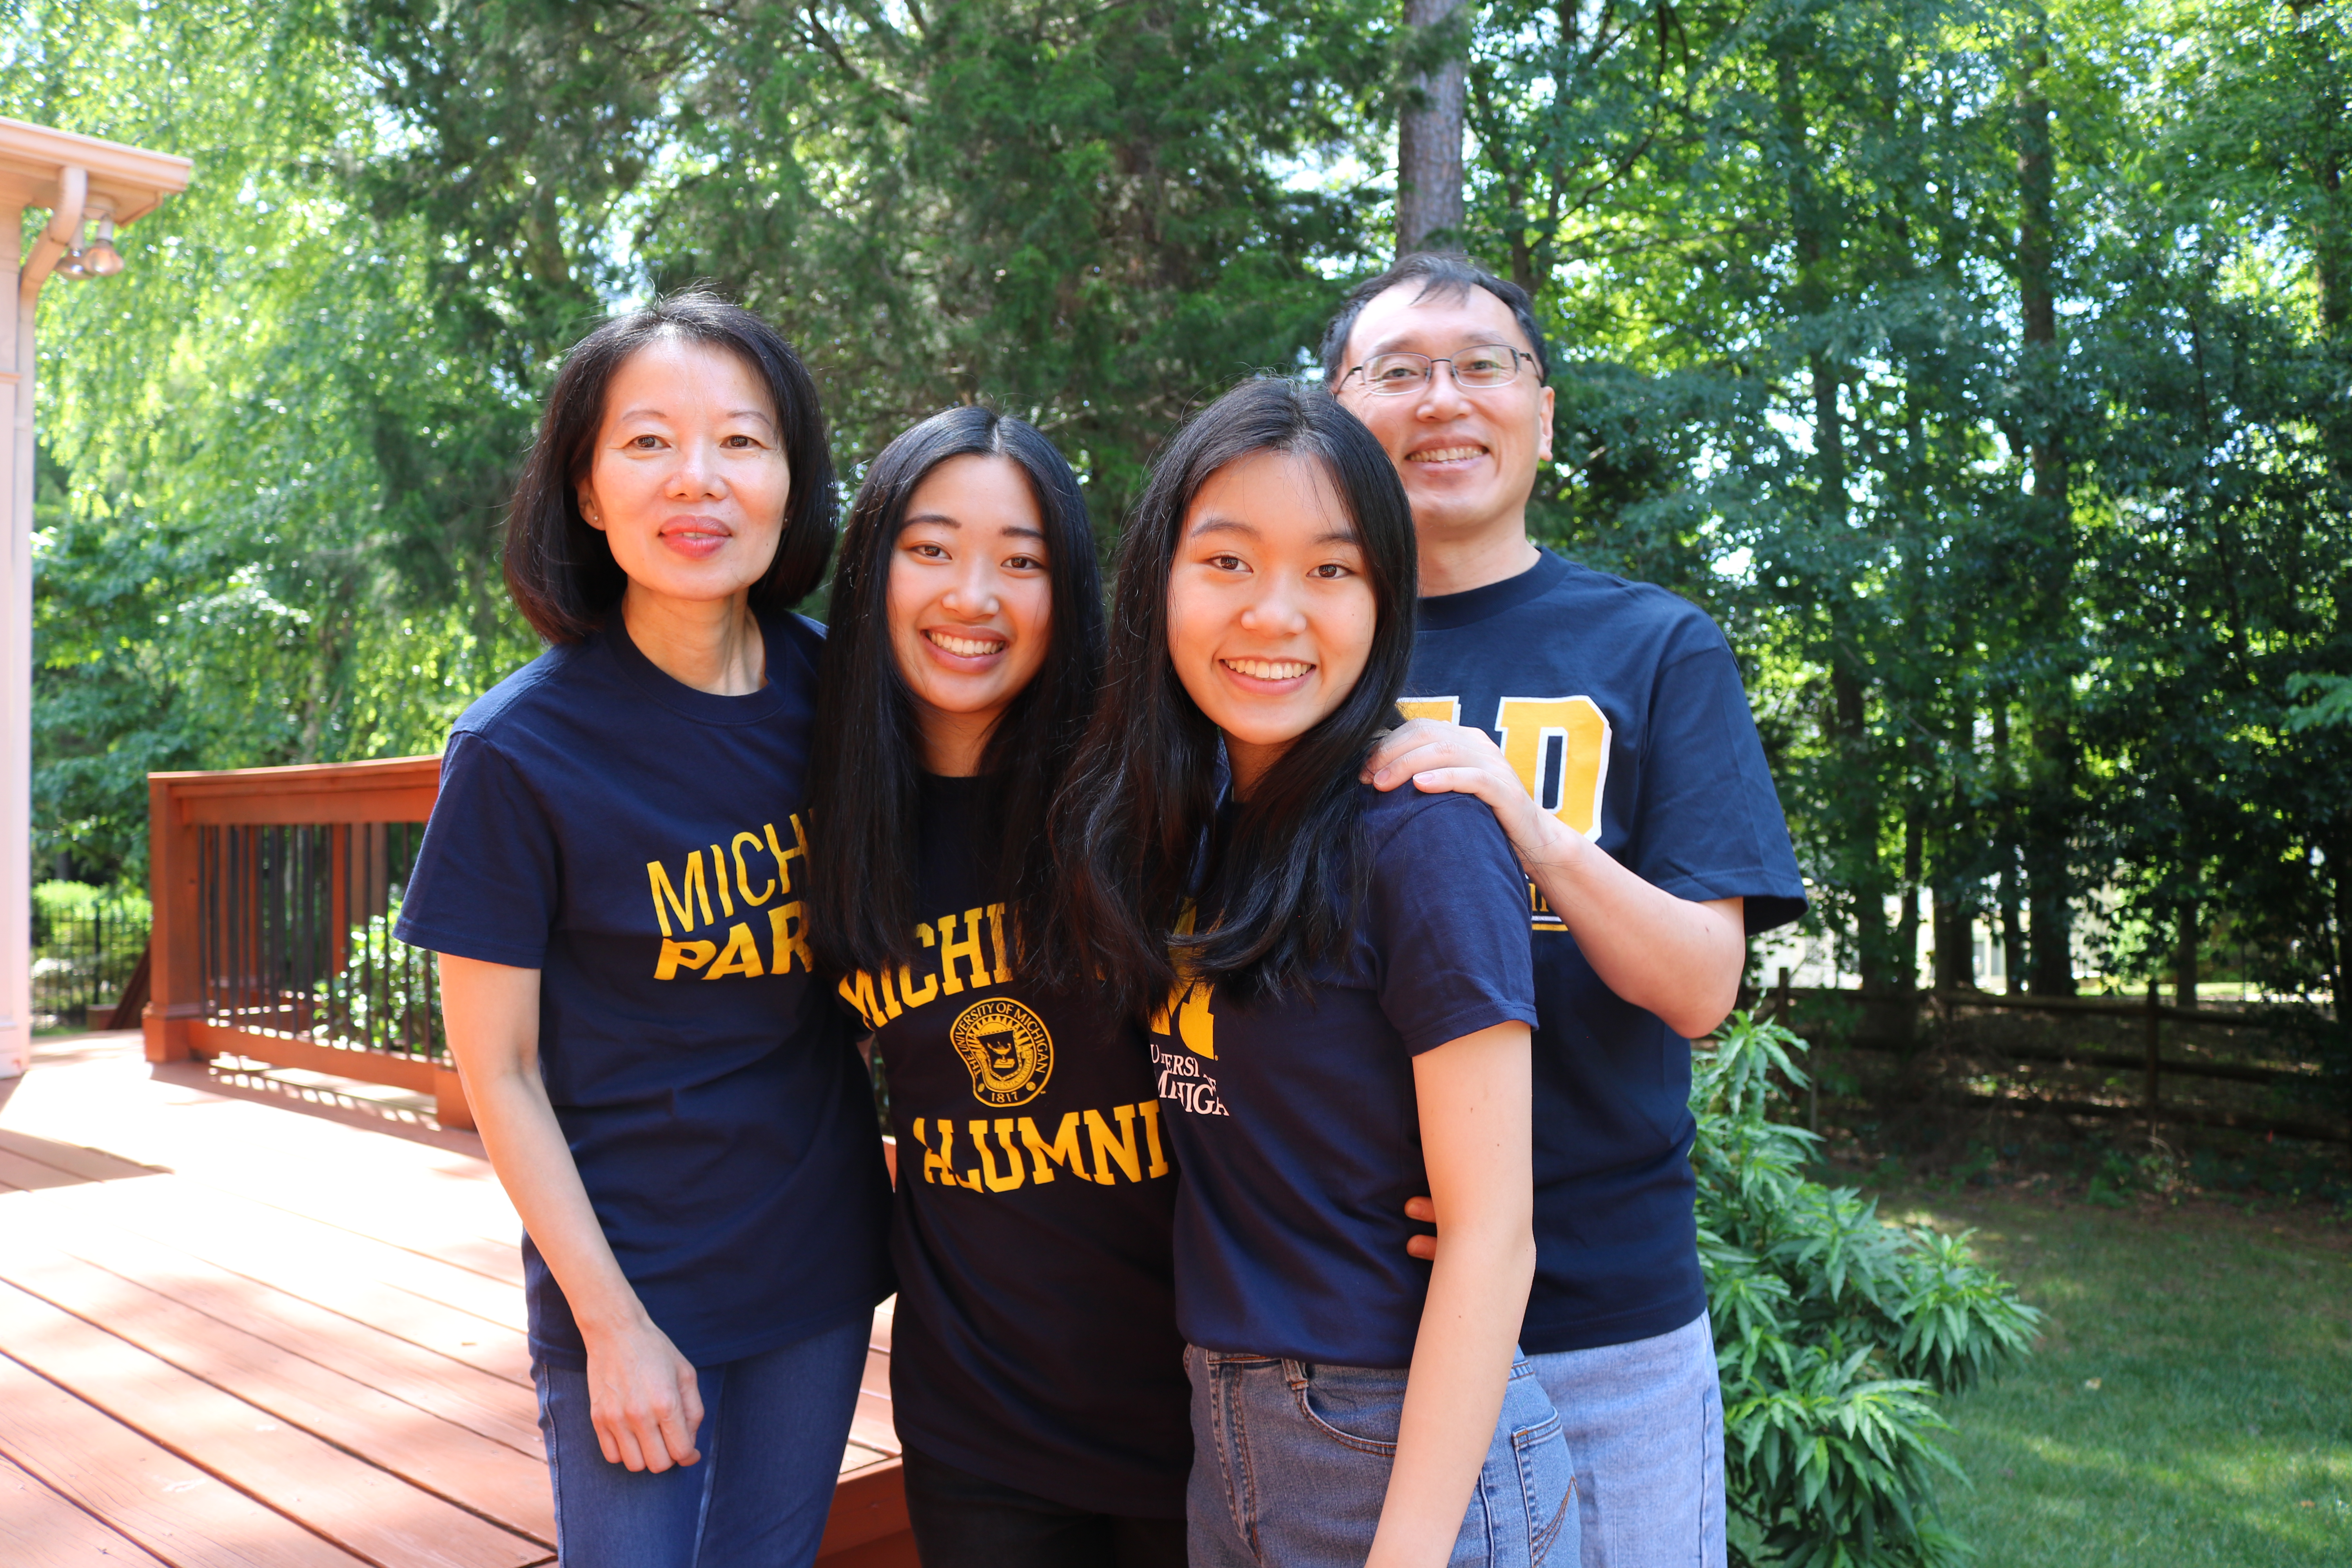
\includegraphics[width=0.4\textwidth,height=\textheight]{fam.JPG}

\includegraphics[width=0.25\textwidth,height=\textheight]{headshot.jpg}

\textbf{Fun Facts!}
- I am from Ann Arbor, MI, but throughout my life, I have also lived in Charlotte, NC and Taipei, Taiwan.
- I come from a family of Wolverines! Both of my parents also attended graduate school at Michigan, and my younger sister is starting her freshman year this fall. GO BLUE!
- In my free time, I love to spend time outdoors, whether that is hiking, camping, or taking pictures of scenery. Check out some of the pictures I took: \url{https://vsco.co/winniferchen/gallery}
- I really enjoy rewatching music videos and performances by my favorite kpop groups. One of my dreams is to go to a kpop concert one day and sit in the very front section.
- Immersing myself in the world of kdramas is another way for me to wind down and relax after a long day.
- Something that I want to do more this year is trying new recipes and cooking more.

\includegraphics[width=0.23\textwidth,height=\textheight]{dtw.png}
\includegraphics[width=0.25\textwidth,height=\textheight]{belleisle.png}
\includegraphics[width=0.25\textwidth,height=\textheight]{econ.png}
\includegraphics[width=0.25\textwidth,height=\textheight]{christmas.JPG}

\hypertarget{jalal-mawri}{%
\section{Jalal Mawri}\label{jalal-mawri}}

Current Master of Business Analytics student at the Ross School of Business

\includegraphics[width=0.25\textwidth,height=\textheight]{jalal1.jpg}
\includegraphics[width=0.25\textwidth,height=\textheight]{jalal2.jpg}
\includegraphics[width=0.25\textwidth,height=\textheight]{jalal3.jpg}

\textbf{Background}

I was born and raised in Yemen, the old city of Sana'a, and I left the country in 2013 with my family and immigrated to the United States. I grew up playing Football, a.k.a soccer, and my favorite team was and still is Manchester United.

\textbf{Education}

\begin{itemize}
\tightlist
\item
  I graduated from the University of Michigan with High Honors in Biology and International Studies.
\item
  During my first two years as an undergraduate student I had the opportunity to work on a research project at the Medical School where we researched preventive medical treatments for strokes.
\item
  During my senior year I wrote my thesis on the current civil war in Yemen, and I researched the Islamic Movement of Ansar Allah which is currently leading the political scene in Yemen and the Arabian Peninsula.
\end{itemize}

\textbf{Professional Experience}

\begin{itemize}
\tightlist
\item
  After graduating I interned for the Muslim Public Affairs Council, and worked on a project that persuaded the Biden Administration to enforce the reopening of Sana's Airport and push for a peace resolution between the parties involved in the war.
\item
  After my internship, I started to work as a Data Analyst for Amazon.
\item
  My plan after I graduate from Ross is to go back to Amazon and work as Business Intelligence Engineer.
\end{itemize}

\textbf{Publications}

Mawri, Jalal. ``Ansar Allah in Yemen: History and Ideology.'' Deep Blue Repositories, 1 Aug.~2021, \url{https://deepblue.lib.umich.edu/handle/2027.42/169403}.

Venugopal J, Wang J, Mawri J, Guo C, Eitzman D. Interleukin-1 receptor inhibition reduces stroke size in a murine model of sickle cell disease. Haematologica. 2021 Sep 1;106(9):2469-2477. doi: 10.3324/haematol.2020.252395. PMID: 32817286; PMCID: PMC8409048.

\hypertarget{footnotes-and-citations}{%
\chapter{Footnotes and citations}\label{footnotes-and-citations}}

\hypertarget{footnotes}{%
\section{Footnotes}\label{footnotes}}

Footnotes are put inside the square brackets after a caret \texttt{\^{}{[}{]}}. Like this one \footnote{This is a footnote.}.

\hypertarget{citations}{%
\section{Citations}\label{citations}}

Reference items in your bibliography file(s) using \texttt{@key}.

For example, we are using the \textbf{bookdown} package \citep{R-bookdown} (check out the last code chunk in index.Rmd to see how this citation key was added) in this sample book, which was built on top of R Markdown and \textbf{knitr} \citep{xie2015} (this citation was added manually in an external file book.bib).
Note that the \texttt{.bib} files need to be listed in the index.Rmd with the YAML \texttt{bibliography} key.

The RStudio Visual Markdown Editor can also make it easier to insert citations: \url{https://rstudio.github.io/visual-markdown-editing/\#/citations}

\hypertarget{blocks}{%
\chapter{Blocks}\label{blocks}}

\hypertarget{equations}{%
\section{Equations}\label{equations}}

Here is an equation.

\begin{equation} 
  f\left(k\right) = \binom{n}{k} p^k\left(1-p\right)^{n-k}
  \label{eq:binom}
\end{equation}

You may refer to using \texttt{\textbackslash{}@ref(eq:binom)}, like see Equation \eqref{eq:binom}.

\hypertarget{theorems-and-proofs}{%
\section{Theorems and proofs}\label{theorems-and-proofs}}

Labeled theorems can be referenced in text using \texttt{\textbackslash{}@ref(thm:tri)}, for example, check out this smart theorem \ref{thm:tri}.

\begin{theorem}
\protect\hypertarget{thm:tri}{}\label{thm:tri}For a right triangle, if \(c\) denotes the \emph{length} of the hypotenuse
and \(a\) and \(b\) denote the lengths of the \textbf{other} two sides, we have
\[a^2 + b^2 = c^2\]
\end{theorem}

Read more here \url{https://bookdown.org/yihui/bookdown/markdown-extensions-by-bookdown.html}.

\hypertarget{callout-blocks}{%
\section{Callout blocks}\label{callout-blocks}}

The R Markdown Cookbook provides more help on how to use custom blocks to design your own callouts: \url{https://bookdown.org/yihui/rmarkdown-cookbook/custom-blocks.html}

\hypertarget{sharing-your-book}{%
\chapter{Sharing your book}\label{sharing-your-book}}

\hypertarget{publishing}{%
\section{Publishing}\label{publishing}}

HTML books can be published online, see: \url{https://bookdown.org/yihui/bookdown/publishing.html}

\hypertarget{pages}{%
\section{404 pages}\label{pages}}

By default, users will be directed to a 404 page if they try to access a webpage that cannot be found. If you'd like to customize your 404 page instead of using the default, you may add either a \texttt{\_404.Rmd} or \texttt{\_404.md} file to your project root and use code and/or Markdown syntax.

\hypertarget{metadata-for-sharing}{%
\section{Metadata for sharing}\label{metadata-for-sharing}}

Bookdown HTML books will provide HTML metadata for social sharing on platforms like Twitter, Facebook, and LinkedIn, using information you provide in the \texttt{index.Rmd} YAML. To setup, set the \texttt{url} for your book and the path to your \texttt{cover-image} file. Your book's \texttt{title} and \texttt{description} are also used.

This \texttt{gitbook} uses the same social sharing data across all chapters in your book- all links shared will look the same.

Specify your book's source repository on GitHub using the \texttt{edit} key under the configuration options in the \texttt{\_output.yml} file, which allows users to suggest an edit by linking to a chapter's source file.

Read more about the features of this output format here:

\url{https://pkgs.rstudio.com/bookdown/reference/gitbook.html}

Or use:

\begin{Shaded}
\begin{Highlighting}[]
\NormalTok{?bookdown}\SpecialCharTok{::}\NormalTok{gitbook}
\end{Highlighting}
\end{Shaded}


  \bibliography{book.bib,packages.bib}

\end{document}
